\RequirePackage[l2tabu, orthodox]{nag}	% To be warned of outdated commands
\documentclass[paper=a4, 12pt]{scrartcl}
\usepackage{fontspec}
\usepackage{setspace}			% For line spacing
\usepackage[usenames,dvipsnames]{color}	% For colorful text
\usepackage{microtype}			% For nicer spacing
\usepackage{graphicx}
\usepackage{bigfoot}
%\usepackage{siunitx}			% For units

\usepackage[colorlinks=true,
        linkcolor=black,
        citecolor=black,
        filecolor=black,
        urlcolor=black,
        pdfusetitle]{hyperref}	% Links and URLs
\urlstyle{rm}					% URLs are written in roman instead of typewriter

\frenchspacing					% No extended space after sentences
\clubpenalty = 10000
\widowpenalty = 10000
\displaywidowpenalty = 10000

\setromanfont{Linux Libertine O}
\setsansfont{Linux Biolinum O}

\newcommand{\xxx}[1]{\textbf{\textcolor{red}{#1}}}	% Emphasizing parts to do




% % % % % % % % % % % % % % Heeere we go! % % % % % % % % % % % % % % %

\begin{document}

\title{Report}
\subtitle{INF-9380}
\author{Mathias Bockwoldt}
\date{20.05.2016}

\maketitle

\onehalfspacing

\section{ChIP-Seq SLURM workflow}

All files for this part are in the folder \texttt{chipseq-part}.

\paragraph{1. Bowtie and MPI} All files for this part are in the folder \texttt{ex1\_bowtie}.

I ran bowtie five times in serial mode to get a baseline for the execution time. Afterwards I ran bowtie using MPI as shown in the example script with one to 16 cores five times each. Everything was run on a single node with all 16 cores allocated to my script. Hence, there should not have been any delay by inter-node data transmission. The script for running bowtie with and without MPI is given in \texttt{run.slurm} (calling the MPI script in a loop) and \texttt{mpirun\_script.sh} (calling bowtie with MPI). The runtimes were measured by the \texttt{time} command and saved in \texttt{times.ods}. As the average times varyied quite heavily, I chose the minimum time of five calls for an estimate of the runtime. The speedup is shown in fig \ref{fig:chipseq-bowtie} using \texttt{real} times.

\begin{figure}[ht]
  \centering
    %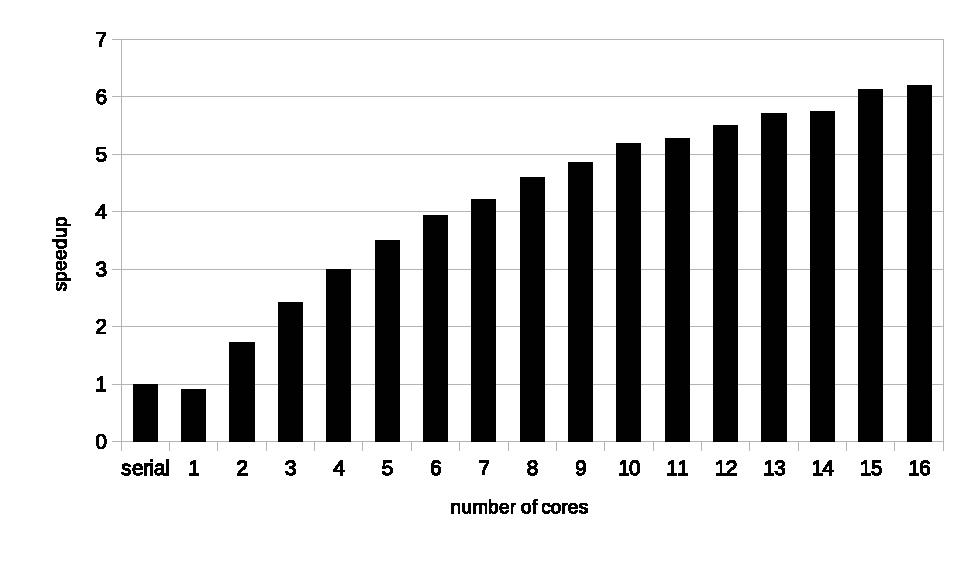
\includegraphics[width=0.5\textwidth]{chipseq-bowtie}
  \caption{The speedup of bowtie with MPI. Serial is bowtie without MPI and is set to 1. The MPI with only one processor has a negative speedup (lower than 1) due to the overhead of parallelisation.}
  \label{fig:chipseq-bowtie}
\end{figure}

The speedup is as expected. The execution gets faster with each additional core, but the increase in speed declines with the number of cores due to the parallelizing overhead. When using more cores, the file must be split into more chunks, more processes must be spawned and more result files must be concatenated after execution. With few processes, this pays off, but the more processes are spawned, the less pronounced is the speedup.

A \texttt{diff} result of the output file of the serial bowtie and bowtie using MPI with 16 cores shows that the file contents themselves are identical. Only the header lines repeat (one header for each process). This is easily solveable for example using awk to remove the excessive headers\footnote{\verb\awk 'NR <= 3 || !/^@/'\}.

\paragraph{2. -- 5. SLURM scripts} All serial files are in the folder \texttt{ex2\_serial} and the parallelized files (using \texttt{arrayrun}) are in the folder \texttt{ex3\_parallel}.

SLURM scripts were written to follow the workflow given in the course. This resulted in eleven scripts plus one for preparation of the data and one R script. Firstly, all scripts were run ones with generous memory and time demands to find out the actual memory consumption and runtime that were used to adjust the sbatch directives accordingly.


\section{Differences between two VCF files}



\section{Galaxy Docker}



\end{document}
